% 第2章第2节：线性泛函的表示（积分读取与点值读取、Riesz表示、有限观测与坐标表示）。

\section{线性泛函的表示}
\label{sec:lfo-functional-representation}

本节固定标量输出，研究一个读数规则怎样写成积分权重或空间中的一个方向。顺序上先检查读数规则对空间元素是否有良定义、是否连续，再讨论表示；表示公式以这些条件为前提，不能反过来替它们作证。

\subsection{积分读取与点值读取}
\label{sec:lfo-point-evaluation}

\paragraph{加权积分读取}
最常见的读数是加权平均：给定权重$g$，读出$\int fg\,d\mu$。在测度空间$(\Omega,\mathcal F,\mu)$上取$1\leq p\leq\infty$，并设$q$是共轭指数，即$1/p+1/q=1$（$p=1$时$q=\infty$，$p=\infty$时$q=1$）。对$g\in L^q(\mu)$，令
\begin{equation}
 L_g(f)=\int_\Omega fg\,d\mu\qquad(f\in L^p(\mu)).
 \label{eq:lfo-integral-reading}
\end{equation}
第~\ref{sec:fs-holder-minkowski}节的Hölder不等式给出$|L_g(f)|\leq\int|fg|\,d\mu\leq\|f\|_p\|g\|_q$，所以积分是有限的，$L_g$是有界线性泛函，且$\|L_g\|\leq\|g\|_q$。第~\ref{sec:lfo-lp-dual}节将证明，在$\sigma$有限测度与$1\leq p<\infty$的条件下这里其实是等号。

$L_g$作用在等价类上是合理的：若$f=\tilde f$几乎处处成立，则$fg=\tilde fg$几乎处处成立，两者积分相同，所以$L_g$的值不依赖代表的选取。这一点看似平凡，却正是积分读取能够在$L^p$上使用的原因。

举一个可以复算的例子。在$L^2(0,1)$上取$g=\mathbf 1_{[0,1/2]}$，$L_g(f)=\int_0^{1/2}f\,dt$读出前半段的累计。Hölder不等式给出$\|L_g\|\leq\|g\|_2=1/\sqrt2$；取$f=g$，则$L_g(g)=1/2$而$\|g\|_2=1/\sqrt2$，比值正好是$1/\sqrt2$，所以$\|L_g\|=1/\sqrt2$。同一规则在$C([0,1])$的一致范数下的范数是$1/2$（取$f\equiv1$），两个数不同，因为输入误差的衡量方式不同。

\paragraph{连续函数的点值读取}
另一类读数是读出某一点的值。设$K$是紧致度量空间，$x\in K$固定。在$C(K)$上配一致范数，令$\delta_x(f)=f(x)$，称为在$x$处的\term{点值泛函}（point evaluation functional）。由$|f(x)|\leq\sup_K|f|=\|f\|_\infty$，$\delta_x$是有界线性泛函，$\|\delta_x\|\leq1$；取$f\equiv1$得$\|\delta_x\|=1$。

两种读数都输出一个标量，但依靠的空间结构不同：积分读取依靠积分对零测集不敏感，点值读取依靠一致范数对每一点都有控制。把点值读取搬到积分空间中，这两种结构就发生冲突。

\paragraph{等价类上没有点值}
在Lebesgue测度下的$L^p(0,1)$中，单点$\{x_0\}$的测度为零。改变一个函数在$x_0$处的值，得到的函数与原函数几乎处处相等，属于同一个等价类，例如$f$与$f+\mathbf 1_{\{x_0\}}$。同一个等价类在$x_0$处可以有任何值，所以“读出$x_0$处的值”在$L^p$上根本没有良定义，谈不上是否有界。

\paragraph{窄尖峰：连续代表也不够}
或许可以只考虑连续函数，因为连续代表若存在则唯一。但即使把对象限制在$C([0,1])$中、用$L^2$范数衡量误差，点值仍然不受控制。取贴着左端点、宽为$1/n$、高为$1$的尖峰
\[
 \tau_n(t)=\max(1-nt,\,0)\qquad(t\in[0,1]).
\]
它连续，$\delta_0(\tau_n)=\tau_n(0)=1$，而直接积分得
\[
 \|\tau_n\|_2^2=\int_0^{1/n}(1-nt)^2\,dt=\frac{1}{3n}\longrightarrow0 .
\]
图~\ref{fig:lfo-point-spike}画出了$n=4,10,25$三个尖峰：$L^2$范数从约$0.289$降到约$0.115$，左端点的值始终是$1$。所以不存在常数$C$使$|f(0)|\leq C\|f\|_2$对一切连续$f$成立，点值泛函在$(C([0,1]),\|\cdot\|_2)$上无界。

\begin{figure}[!htb]
  \centering
  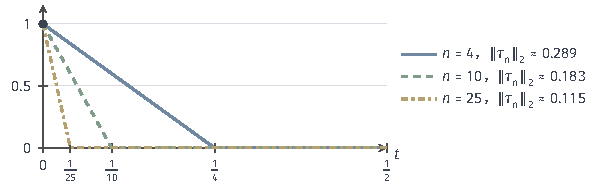
\includegraphics[width=101.7mm]{figures/02-abstract-mathematics/03-function-spaces/tikz/c2-point-spike/figure.pdf}
  \caption{窄尖峰使点值不受$L^2$范数控制。尖峰$\tau_n(t)=\max(1-nt,0)$在$n=4,10,25$时的图像（蓝实线、绿虚线、黄点划线）。左端点的值恒为$1$（黑点），而$\|\tau_n\|_{L^2(0,1)}=1/\sqrt{3n}$随$n$增大趋于零。}
  \label{fig:lfo-point-spike}
\end{figure}

\paragraph{原子测度改变结论}
上面的困难来自单点的测度为零。若测度在$x_0$处有正的质量，结论就会改变。在$[0,1]$上取$\mu=\lambda+\delta_{x_0}$，其中$\lambda$是Lebesgue测度，$\delta_{x_0}$是集中在$x_0$的单位质量。此时$\mu(\{x_0\})=1$，改变$x_0$处的值会改变等价类，于是$f(x_0)$对$L^2(\mu)$的元素有良定义，并且
\[
 |f(x_0)|^2=\int_{\{x_0\}}|f|^2\,d\mu\leq\int|f|^2\,d\mu=\|f\|_{L^2(\mu)}^2 .
\]
正测度的单点原子与零测单点必须区分。一般的积分空间不支持点值读取；第~\ref{chap:rkhs}章将专门研究点值读取连续的Hilbert函数空间，第~\ref{sec:sob-embedding}节则说明控制导数能在什么条件下恢复点值的连续性。

\subsection{Hilbert空间中的Riesz表示}
\label{sec:lfo-riesz}

\paragraph{每个方向给出一个读数}
在Hilbert空间$H$中，任取$h\in H$，令$L_h(f)=\langle h,f\rangle$。按全书的约定，内积对第二个变量线性，所以$L_h$是线性泛函。Cauchy--Schwarz不等式给出$|L_h(f)|\leq\|h\|\,\|f\|$，即$\|L_h\|\leq\|h\|$；$h\neq0$时取$f=h/\|h\|$，得$L_h(f)=\|h\|$，于是$\|L_h\|=\|h\|$。每个方向都是一个读数规则，读数的范数等于方向的长度。

反过来的问题更有用：给定一个有界线性读数$L$，是否一定存在方向$h$，使读数就是与$h$做内积？若是，就可以用空间中的几何（正交、投影、长度）来研究读数。

\paragraph{核与正交方向}
先观察一个非零有界线性泛函$L$的核$N=\ker L=\{f:L(f)=0\}$。它是线性子空间；又因为$L$连续，若$f_n\in N$且$f_n\to f$，则$L(f)=\lim L(f_n)=0$，所以$N$是闭子空间。$N$还“只差一维”：任取$w\notin N$，每个$f$都可以写成
\[
 f=\Bigl(f-\frac{L(f)}{L(w)}w\Bigr)+\frac{L(f)}{L(w)}w ,
\]
括号中的元素在$L$下的值为零，属于$N$。所以$H=N+\operatorname{span}\{w\}$。若进一步把$w$取在$N$的正交补中，读数$L(f)$就只取决于$f$沿$w$方向的分量，这正是表示向量的来源。由此得到的结论称为\term{Riesz表示定理}（Riesz representation theorem）。

\begin{theorem}[Riesz表示定理]
\label{thm:lfo-riesz}
设$H$是Hilbert空间，$L:H\to\mathbb F$是有界线性泛函。则存在唯一的$h_L\in H$，使
\begin{equation}
 L(f)=\langle h_L,f\rangle\qquad(f\in H),
 \label{eq:lfo-riesz}
\end{equation}
并且$\|L\|=\|h_L\|$。
\end{theorem}

证明分三步：用投影找出与核正交的方向，用这个方向写出表示，再验证唯一性与范数等式。

\begin{proof}
$L=0$时取$h_L=0$。下设$L\neq0$，于是闭子空间$N=\ker L$不是全空间。

\emph{第一步：找与核正交的方向。}取$v$使$L(v)\neq0$。由第~\ref{sec:fs-projection}节的正交投影定理，$v=P_Nv+w$，其中$P_Nv\in N$，$w=v-P_Nv\perp N$。由$L(w)=L(v)-L(P_Nv)=L(v)\neq0$知$w\neq0$。

\emph{第二步：写出表示。}对任意$f\in H$，前面已说明$f-\frac{L(f)}{L(w)}w\in N$，它与$w$正交：
\[
 0=\Bigl\langle w,\ f-\frac{L(f)}{L(w)}w\Bigr\rangle=\langle w,f\rangle-\frac{L(f)}{L(w)}\|w\|^2 .
\]
这里用到内积对第二个变量线性。解出$L(f)=\frac{L(w)}{\|w\|^2}\langle w,f\rangle$。令
\begin{equation}
 h_L=\frac{\overline{L(w)}}{\|w\|^2}\,w ,
 \label{eq:lfo-riesz-direction}
\end{equation}
由于内积对第一个变量共轭线性，$\langle h_L,f\rangle=\frac{L(w)}{\|w\|^2}\langle w,f\rangle=L(f)$。

\emph{第三步：唯一性与范数。}若$h,h'$都满足式~\eqref{eq:lfo-riesz}，则$\langle h-h',f\rangle=0$对一切$f$成立，取$f=h-h'$得$h=h'$。范数等式正是本小节开头对$L_h$的计算。
\end{proof}

式~\eqref{eq:lfo-riesz-direction}中的共轭在实空间中消失；在复空间中，它使对应$L\mapsto h_L$是共轭线性的：$h_{\alpha L}=\bar\alpha h_L$。这是内积对第一个变量共轭线性这一约定的直接后果。

\paragraph{读数的几何}
图~\ref{fig:lfo-riesz-kernel}在实平面的二维截面上画出了这个构造。核$N$是一条过原点的直线，表示向量$h_L$与它垂直；读数相等的点组成平行于$N$的直线，读数每增加$\|h_L\|^2$，水平线沿$h_L$方向平移一个$\|h_L\|$的距离。任何$f$都分解为$N$中的分量与沿$h_L$的分量，前者对读数没有贡献，后者的长度决定读数。读数大的方向就是$h_L$本身，这也解释了$\|L\|=\|h_L\|$：在单位球上，沿$h_L$方向的单位向量读到的值最大。

\begin{figure}[!htb]
  \centering
  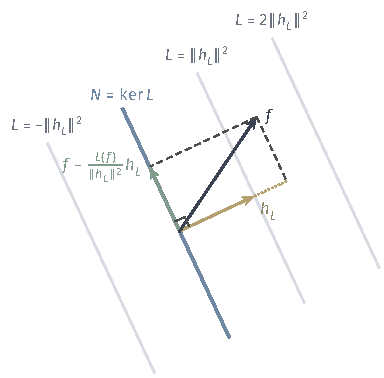
\includegraphics[width=65.1mm]{figures/02-abstract-mathematics/03-function-spaces/tikz/c2-riesz-kernel/figure.pdf}
  \caption{Riesz表示的几何示意（实空间中的二维截面）。核$N=\ker L$（蓝线）是闭子空间，表示向量$h_L$（黄）与之正交；灰线是读数$L=c$的水平集，平行于$N$。元素$f$减去沿$h_L$的分量$\frac{L(f)}{\|h_L\|^2}h_L$后落入$N$（绿），因此读数只由$f$沿$h_L$方向的分量决定。}
  \label{fig:lfo-riesz-kernel}
\end{figure}

\paragraph{$L^2$中的读数与方向}
在$L^2(0,1)$中，几个熟悉的读数对应的方向都可以直接写出。整体平均$L(f)=\int_0^1f\,dt=\langle1,f\rangle$对应常数$h_L=1$，$\|L\|=1$。前半段平均$L(f)=2\int_0^{1/2}f\,dt$对应$h_L=2\cdot\mathbf 1_{[0,1/2]}$，$\|L\|=\|h_L\|_2=2\cdot(1/2)^{1/2}=\sqrt2$。加权读数$L(f)=\int_0^1tf(t)\,dt$对应$h_L(t)=t$，$\|L\|=(\int_0^1t^2\,dt)^{1/2}=1/\sqrt3$。正交展开中的第$k$个系数$f\mapsto\langle e_k,f\rangle$对应$h_L=e_k$。抽象的读数规则由此变成了与一个固定函数的比较，读数的大小就是$f$与这个函数的相关程度。

\paragraph{表示以有界为前提}
Riesz表示定理需要两个前提，缺一不可。第一，$L$必须已经有界。在$C([0,1])$上配$L^2$内积，点值$\delta_0$无界；它也确实没有表示函数：若有连续$h$使$f(0)=\int_0^1hf\,dt$对一切连续$f$成立，代入尖峰$\tau_n$，左端恒为$1$，右端的绝对值不超过$\|h\|_2\|\tau_n\|_2\to0$，矛盾。定理不能替点值读取证明连续性，连续性必须事先单独检验。

第二，空间必须完备。仍在$C([0,1])$上配$L^2$内积，读数$L(f)=\int_0^{1/2}f\,dt$满足$|L(f)|\leq\|f\|_2/\sqrt2$，是有界的。在完备的$L^2(0,1)$中它的表示方向是$\mathbf 1_{[0,1/2]}$，但这个函数没有连续代表，不在$C([0,1])$中。所以在不完备的内积空间里，有界读数可以没有表示向量；证明中用到的正交投影定理依赖完备性，此处失效。

最后，Riesz表示只处理标量输出。输出为向量的观测，例如同时读出两个端点值$(f(0),f(1))$，要逐个分量作为标量泛函处理，各分量分别有自己的表示方向（若它们有界），不能未经说明就当作一个泛函。

\subsection{有限观测与坐标表示}
\label{sec:lfo-finite-observations}

实际中我们只能对函数做有限次读数，并且常把候选函数限制在一个有限维空间里。本小节说明在这种设定下，读数、坐标和函数之间怎样用矩阵联系，以及有限条读数能否唯一确定一个函数。

\paragraph{观测矩阵}
设候选函数属于有限维子空间$V=\operatorname{span}\{\varphi_1,\ldots,\varphi_m\}$，其中$\varphi_1,\ldots,\varphi_m$线性无关，每个$f\in V$唯一地写成$f=\sum_{j=1}^mc_j\varphi_j$，系数向量记为$\bm c=(c_1,\ldots,c_m)^{\top}$。再设$L_1,\ldots,L_n$是$V$上的线性读数。由线性，
\[
 L_i(f)=\sum_{j=1}^mc_jL_i(\varphi_j)\qquad(i=1,\ldots,n).
\]
令$\bm A\in\mathbb F^{n\times m}$，$\bm A_{i,j}=L_i(\varphi_j)$，称为\term{观测矩阵}（observation matrix），则读数向量$\bm r=(L_1(f),\ldots,L_n(f))^{\top}$满足
\begin{equation}
 \bm r=\bm A\bm c .
 \label{eq:lfo-observation-matrix}
\end{equation}
矩阵的第$i$行是第$i$条读数规则在各个基函数上的取值，第$j$列是第$j$个基函数在全部读数下留下的记录。点值读数给出$\bm A_{i,j}=\varphi_j(x_i)$，积分读数给出$\bm A_{i,j}=\int\varphi_jg_i\,d\mu$；代入之前仍须核对每条读数在$V$上有良定义。

\paragraph{仿射函数的两次读数}
取$V$为$[0,1]$上的仿射函数，基为$\varphi_1=1$、$\varphi_2=t$，$f=c_1+c_2t$。读$f(0)$与$f(1)$时，
\[
 \bm A=\begin{bmatrix}1&0\\1&1\end{bmatrix},\qquad
 \begin{bmatrix}f(0)\\f(1)\end{bmatrix}=\bm A\begin{bmatrix}c_1\\c_2\end{bmatrix}.
\]
$\bm A$可逆，由$c_1=f(0)$、$c_2=f(1)-f(0)$恢复系数。若只读$f(0)$，$\bm A=[1\ \ 0]$，第二列为零：斜率方向在记录中完全看不见。若改读$f(0)$与整体平均$\int_0^1f\,dt$，第二行变为$(1,1/2)$，矩阵仍可逆。图~\ref{fig:lfo-observation-matrix}(a)(b)对比了一次与两次点值读数的情形。

\paragraph{非标准正交基下的Gram矩阵}
坐标向量$\bm c$与函数$f$一一对应，但坐标的欧氏长度一般不是函数的范数。在内积空间中，记\term{Gram矩阵}（Gram matrix）$\bm G_{j,k}=\langle\varphi_j,\varphi_k\rangle$，则对$f=\sum_jc_j\varphi_j$、$u=\sum_kd_k\varphi_k$有
\[
 \langle f,u\rangle=\sum_{j,k}\bar c_jd_k\langle\varphi_j,\varphi_k\rangle=\bm c^{\mathsf H}\bm G\bm d ,
\]
其中$\bm c^{\mathsf H}$是共轭转置，实情形即$\bm c^{\top}$。只有基标准正交时$\bm G=\bm I$，函数内积才等于系数内积。

仍以$L^2(0,1)$中的基$1,t$为例，$\bm G=\bigl[\begin{smallmatrix}1&1/2\\1/2&1/3\end{smallmatrix}\bigr]$。函数$f=t-1/2$的系数为$\bm c=(-1/2,1)^{\top}$，于是$\|f\|_2^2=\bm c^{\top}\bm G\bm c=\tfrac14-\tfrac12+\tfrac13=\tfrac1{12}$，与直接积分$\int_0^1(t-1/2)^2\,dt=1/12$一致；而系数的欧氏长度平方是$5/4$，差了十五倍。在坐标中计算误差或正交性时，必须带上$\bm G$。

\paragraph{唯一恢复的条件}
读数能否唯一确定候选空间中的函数，归结为观测矩阵的列是否线性无关。

\begin{theorem}[有限维候选的唯一恢复]
\label{thm:lfo-finite-recovery}
设$V$与$L_1,\ldots,L_n$如上，$\bm A$为观测矩阵。则读数向量唯一确定$V$中的函数，当且仅当$\bm A$满列秩，即$\operatorname{rank}\bm A=m$。特别地，这要求$n\geq m$。
\end{theorem}

\begin{proof}
两个候选$f=\sum c_j\varphi_j$与$u=\sum d_j\varphi_j$给出相同读数，当且仅当$\bm A(\bm c-\bm d)=\bm 0$。所以读数唯一确定函数，当且仅当$\bm A\bm z=\bm 0$只有零解，即$\bm A$的$m$列线性无关；这又等价于秩为$m$，而秩不超过行数$n$。
\end{proof}

结论严格限定在给定的候选空间$V$上。图~\ref{fig:lfo-observation-matrix}(c)把候选扩大到二次多项式：基$1,t,t(t-1)$下，两次点值读数的观测矩阵为$\bigl[\begin{smallmatrix}1&0&0\\1&1&0\end{smallmatrix}\bigr]$，第三列为零，函数$t(t-1)$在$t=0,1$处都等于零，在两次读数中看不见。于是$1+t+s\,t(t-1)$对一切$s$给出相同的记录。

\begin{figure}[!htb]
  \centering
  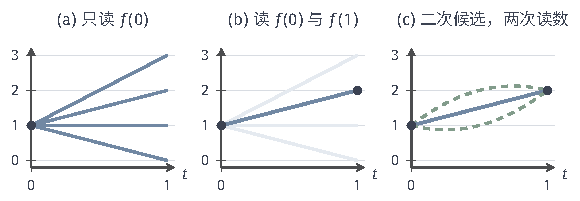
\includegraphics[width=98.2mm]{figures/02-abstract-mathematics/03-function-spaces/tikz/c2-observation-matrix/figure.pdf}
  \caption{有限读数能否确定候选函数。(a)~仿射候选$f=1+bt$（$b=-1,0,1,2$）都满足$f(0)=1$，一次读数无法区分；(b)~再读$f(1)=2$，只剩$b=1$（深蓝线），观测矩阵满列秩；(c)~候选扩大为二次多项式后，$1+t+s\,t(t-1)$（$s=-2,0,2$）在$t=0,1$处的读数完全相同，方向$t(t-1)$不可见。}
  \label{fig:lfo-observation-matrix}
\end{figure}

\paragraph{无限维中有限读数不够}
若候选空间是无限维的，有限条读数永远不能唯一确定函数。线性映射$f\mapsto(L_1(f),\ldots,L_n(f))$从候选空间映到$\mathbb F^n$；它的核若只含零，就会把一个无限维空间单射地放进$n$维空间，这不可能。所以总有非零的$f$使全部读数为零，加到任何候选上都不改变记录。上面的$t(t-1)$只是这种不可见方向在二次多项式中的具体样子。

本小节只建立空间元素、坐标与读数之间的对应。读数带有噪声或彼此不相容时，$\bm r=\bm A\bm c$可能无解，需要另选拟合准则与误差度量；这属于优化问题，可参考\BookChapterRef{chap:optimization}{卷三“优化问题的定义与基本性质”章}。第~\ref{sec:rkhs-finite-observations}节将在点值连续的核空间中，用Riesz表示方向重新组织有限观测。
